\documentclass[10pt,a4paper]{article}
\usepackage{amsmath,amssymb,amsthm,graphicx}
\usepackage{amsfonts,amssymb,amsmath,amsthm,mathtools,graphicx,bm,xspace,booktabs,array,multirow,dsfont}
\usepackage{enumitem}
\setlist[itemize]{noitemsep}
\setlist[enumerate]{noitemsep}
\usepackage[usenames,dvipsnames]{xcolor}
\definecolor{Gred}{RGB}{219,50,54}
\definecolor{Ggreen}{RGB}{60,186,84}
\definecolor{Gblue}{RGB}{72,133,237}
\definecolor{Gyellow}{RGB}{247,178,16}
\definecolor{ToCgreen}{RGB}{0,128,0}
\definecolor{myGold}{RGB}{231,141,20}
\definecolor{myBlue}{rgb}{0.19,0.41,.65}
\definecolor{myPurple}{RGB}{175,0,124}
\usepackage[colorlinks=true,hypertexnames=false]{hyperref}
\usepackage{tikz}
\usetikzlibrary{arrows.meta,shapes}
\usepackage[framemethod=tikz]{mdframed}
\mdfsetup{roundcorner=4pt,linewidth=.5,innerleftmargin=10pt,innerrightmargin=10pt,innertopmargin=10pt,innerbottommargin=10pt}
\usepackage{thmtools,thm-restate}
\usepackage[no-math]{fontspec}
\newtheorem{theorem}{Theorem}
\newtheorem{lemma}[theorem]{Lemma}
\newtheorem{corollary}[theorem]{Corollary}
\newtheorem{proposition}[theorem]{Proposition}
\newtheorem{claim}[theorem]{Claim}
\newtheorem{fact}[theorem]{Fact}
\newtheorem{techlemma}[theorem]{Technical Lemma}
\theoremstyle{definition}
\newtheorem{definition}[theorem]{Definition}
\theoremstyle{remark}
\newtheorem{remark}[theorem]{Remark}
\newtheorem{example}[theorem]{Example}
\newenvironment{Enumerate}{\begin{enumerate}}{\end{enumerate}}
\newenvironment{Itemize}{\begin{itemize}}{\end{itemize}}
\newcommand{\contour}[2]{#2}
\let\boldm\bm
\newenvironment{nproblem}[1][\unskip]{\medskip\begin{mdframed}\noindent\underline{$#1$ Problem.}\\\noindent}{\end{mdframed}}
\allowdisplaybreaks
\AtBeginDocument{\author{\parbox{.95\textwidth}{\centering Mika G\"o\"os, Pritish Kamath,\\ Katerina Sotiraki, Manolis Zampetakis}}}

\newcommand{\inparen}[1]{\left ( #1 \right )}
\newcommand{\infork}[1]{\left \{ \begin{matrix} #1 \end{matrix} \right .}
\newcommand{\inabs}[1]{\begin{vmatrix} #1 \end{vmatrix}}
\renewcommand{\mod}[1]{~\inparen{\mathrm{mod}~#1}}
\newcommand{\bx}{{\boldm x}}
\def\ceil#1{\mathop{\left\lceil#1\right\rceil}}
\def\abs#1{\left|#1\right|}
\def\p#1{\left(#1\right)}
\def\a#1{\langle#1\rangle}
\def\set#1{\left\{#1\right\}}
\newcommand{\parasc}[1]{\noindent \contour{black}{#1}}
\newcommand{\paragr}[1]{\noindent \textbf{\boldmath #1}}
\newcommand{\F}{\ensuremath{\mathbb{F}}}
\newcommand{\bbF}{\ensuremath{\mathbb{F}}}
\newcommand{\bbZ}{\ensuremath{\mathbb{Z}}}
\newcommand{\calC}{\mathcal{C}}
\newcommand{\calG}{\mathcal{G}}
\newcommand{\calM}{\mathcal{M}}
\newcommand{\calR}{\mathcal{R}}
\newcommand{\calT}{\mathcal{T}}
\newcommand{\calV}{\mathcal{V}}
\renewcommand{\vec}[1]{\boldsymbol{#1}}
\newcommand{\vecf}{\ensuremath{\boldsymbol{f}}}
\newcommand{\vecg}{\ensuremath{\boldsymbol{g}}}
\newcommand{\vech}{\ensuremath{\boldsymbol{h}}}
\newcommand{\vecv}{\ensuremath{\boldsymbol{v}}}
\newcommand{\vecx}{\ensuremath{\boldsymbol{x}}}
\newcommand{\vecy}{\ensuremath{\boldsymbol{y}}}
\newcommand{\vecz}{\ensuremath{\boldsymbol{z}}}
\newcommand{\bit}{\ensuremath{\set{0,1}}}
\DeclareMathOperator*{\poly}{\ensuremath\mathrm{poly}}
\newcommand{\problem}[1]{\ensuremath{\textsc{#1}}\xspace}
\newcommand{\class}[1]{\ensuremath{\mathsf{#1}}\xspace}
\newcommand{\FNP}{\class{FNP}}
\newcommand{\TFNP}{\class{TFNP}}
\newcommand{\PPA}{\class{PPA}}
\newcommand{\PPAp}{\class{PPA}_{{p}}}
\newcommand{\sis}{\problem{SIS}}
\newcommand{\pnum}{p}
\newcommand{\qnum}{q}
\newcommand{\lonelyp}{\ensuremath\textsc{Lonely}_{\pnum}}
\newcommand{\bipartitep}{\ensuremath{\textsc{Bipartite}_{\pnum}}}
\newcommand{\twoMatchingsp}{\ensuremath{\textsc{TwoMatchings}_{\pnum}}}
\newcommand{\sucBipartitep}{\ensuremath{\textsc{SuccinctBipartite}_{\pnum}}}
\newcommand{\leafq}{\ensuremath\textsc{Leaf}_{\qnum}}
\newcommand{\lonelyq}{\ensuremath\textsc{Lonely}_{\qnum}}
\newcommand{\bipartiteq}{\ensuremath{\textsc{Bipartite}_\qnum}}
\newcommand{\leaf}{\ensuremath\textsc{Leaf}}
\newcommand{\lonely}{\ensuremath\textsc{Lonely}}
\newcommand{\bipartite}{\ensuremath{\textsc{Bipartite}}}
\newcommand{\twoMatchings}{\ensuremath{\textsc{TwoMatchings}}}
\newcommand{\sucBipartite}{\ensuremath{\textsc{SuccinctBipartite}}}
\newcommand{\reducible}{\preceq}
\newcommand{\Chevalley}{\ensuremath\textsc{Chevalley}}
\newcommand{\CWT}{CWT\xspace}
\newcommand{\lChevalleyp}{\textsc{GeneralChevalley}_{\pnum}}
\newcommand{\cChevalleyp}{\textsc{ChevalleyWithSymmetry}_{\pnum}}
\newcommand{\eChevalleyp}{\textsc{Chevalley}_{\pnum}}
\newcommand{\lChevalley}{\textsc{GeneralChevalley}}
\newcommand{\cChevalley}{\textsc{ChevalleyWithSymmetry}}
\newcommand{\eChevalley}{\textsc{Chevalley}}
\newcommand{\CW}{\mathsf{CW}}

\providecommand{\bigtimes}{\mathop{\times}\displaylimits}
\providecommand{\bracks}[1]{\left[#1\right]}

\newcommand{\M}{\mathsf M}
\renewcommand{\P}{\mathsf P}
\newcommand{\amp}{\textsf{\upshape\&}}
\newcommand{\bamp}{~\textsf{\upshape\&}~}
\newcommand{\secref}[1]{\hyperref[#1]{\S\ref{#1}}}
\newcommand{\eqnref}[1]{\hyperref[#1]{Eq.~\ref{#1}}}
\title{Classification of modulo-q total-search classes by prime factors via coprime and prime-power reductions}
\author{Mika Göös, Pritish Kamath, Katerina Sotiraki, Manolis Zampetakis}
\date{doi:10.4230/LIPIcs.CCC.2020.19; CC BY 3.0 Unported}
\begin{document}
\maketitle
\noindent\textit{Editorial scope.} One independent composite-modulus classification mechanism,grouping coprime and prime-power reductions with their support. Operator\& is the tagged-input class combination. Concurrent independent Hollender result attributed and not counted separately. No CWT/SIS/application/survey tasks split from this theorem.\par\medskip
\noindent\textit{Allowed standard prerequisites (editorial).}\begin{itemize}
\item TFNP many-one reductions,prime divisibility of binomial coefficients and efficient subset indexing. Exact formal q>=2 and prime-p conventions retained;operator\& defined through tagged-input complete problems,not confused with set intersection. Fact11 binomial congruences and cited efficient subset indexing[31] remain standard prerequisites;full local canonical grouping/indexing/witness arguments and graph equivalences retained. Full37 original references.
\end{itemize}\medskip
\setcounter{section}{1}
\setcounter{subsection}{0}
\setcounter{theorem}{0}
\setcounter{figure}{1}
\subsection{Characterization via Prime Modulus} \label{sec:intro-char}

  We show, in \autoref{sec:characterization}, that every class $\PPA_q$ is built
out of the classes $\PPA_p$ for $p$ a prime. To formalize this result, we
recall the operator `\amp' defined by Buss and
Johnson \cite[\S6]{r13}. For any two syntactic complexity
classes $\M_0$, $\M_1$ with complete problems $S_0$, $S_1$, the class
$\M_0 \bamp \M_1$ is defined via its complete problem $S_0 \bamp S_1$ where, on
input $(x, b) \in \{0, 1\}^* \times \bit$, the goal is to find a solution for
$x$ interpreted as an instance of problem $S_b$. Namely, if $b = 0$ then the output has to be a solution of $S_0$ with
input $x$, and otherwise it has to be a solution of $S_1$ with input $x$.
Intuitively speaking, $\M_1 \bamp \M_2$ combines
the powers of both $\M_1$ and $\M_2$. Note that
$\M_1 \cup \M_2 \subseteq \M_1 \bamp \M_2$. We can now formally
express our characterization result (where $p|q$ is the set of primes $p$
dividing $q$).


\begin{theorem}\label{thm:prime-characterization}
$\PPA_q = \amp_{p|q}\, \PPA_p$.
\end{theorem}


\noindent A special case of \autoref{thm:prime-characterization} is that
$\PPA_{p^k}=\PPA_p$ for every prime power $p^k$. Showing the inclusion
$\PPA_{p^k}\subseteq \PPA_p$ is the crux of our proof. This part of the theorem can be viewed as a total search problem
analog of the counting class result of Beigel and Gill~\cite{r7}
stating that $\mathsf{Mod}_{p^k}\P = \mathsf{Mod}_{p}\P$; ``an unexpected
result'', they wrote at the time. Throughout this paper, we use $q$ to denote any integer $\ge 2$ and $p$ to denote a prime integer.

\paragraph{Concurrent independent work (original attribution)}
We note that a concurrent and independent work by Hollender~\cite{r25} also establishes the structural properties corresponding to the prime-modulus characterization and relative structural-power discussion.

\setcounter{section}{1}
\setcounter{theorem}{5}
\section{\boldmath The class $\PPA_q$}
\label{sec:definitions}

\paragraph{\boldmath Search Problems in $\FNP$ and $\TFNP$.} A search problem
in $\FNP$ is defined by a polynomial time computable relation
$\calR\subseteq \bit^* \times \bit^*$, that is, for every $(x,y)$, it is
possible to decide whether $(x,y) \in \calR$ in $\poly(|x|, |y|)$ time. A
solution to the search problem on input $x$ is a $y$ such that
$|y| = \poly(|x|)$ and $(x,y) \in \calR$. For convenience, define
$\calR(x) \coloneqq \set{y : (x,y) \in \calR}$. A search problem is {\em total}
if for every input $x \in \bit^*$, there exists $y \in \calR(x)$ such that $|y|
\le \poly(|x|)$. $\TFNP$ is the class of all total search problems in $\FNP$.

\paragraph{Reducibility among search problems.} A search problem $\calR_1$ is
{\em Karp-reducible} (or {\em many-one reducible}) to a search problem
$\calR_2$, or $\calR_1 \preceq \calR_2$ for short, if there exist polynomial-time computable functions $f$ and $g$ such that given any instance $x$ of $\calR_1$, $f(x)$ is an instance of $\calR_2$ such that for any $y \in \calR_2(f(x))$, it holds that $g(x, f(x), y) \in \calR_1(x)$.

On the other hand, we say that $\calR_1$ is {\em Turing-reducible} to $\calR_2$, or $\calR_1 \preceq_T \calR_2$ for short, if there exists a polynomial-time oracle Turing machine that on input $x$ to $\calR_1$, makes oracle queries to $\calR_2$, and outputs a $y \in \calR_1(x)$. In this paper, we primarly deal with Karp-reductions, except in Section7.3, where we compare the two different notions of reductions in the context of $\PPA_q$.

\paragraph{\boldmath $\PPA_q$ via complete problems.} We describe several total search problems (parameterized by $q$) that we show to be inter-reducible. $\PPA_q$ is then defined as the set of all search problems reducible to either one of the search problems defined below.

Recall that Boolean circuits take inputs of the form $\bit^n$ and operate using ($\wedge$, $\vee$, $\lnot$) gates. In addition, we'll also consider circuits acting on inputs in $[q]^n$. We interpret the input to be of the form $(\bit^{\ceil{\log q}})^n$, where the circuit will be evaluated only on inputs where each block of $\ceil{\log q}$ bits represents a element in $[q]$. In the case where $q$ is a prime, we could also represent the circuit as $C:\bbF_q^n \to \bbF_q^n$ with arbitrary gates of the form $g: \bbF_q^2 \to \bbF_q$. However, we can simulate any such gate with $\poly(q)$ many $+$ and $\times$ operations (over $\bbF_q$) along with a constant $(1)$ gate. Hence, in the case of prime $q$, we'll assume that such circuits are composed of only $(+, \times, 1)$ gates.\\[1mm]





\noindent
\begin{minipage}{\linewidth}
\begin{definition}
	\label{def:bipartite} \contour{black}{($\bipartite_q$)}\vspace{-5pt}
	\begin{itemize}[leftmargin=2.15cm,itemsep=4pt]
		\item[\slshape Principle:] A bipartite graph with a non-multiple-of-$q$ degree node has another such node.
		\item[\slshape Object:] Bipartite graph $G = (V \cup U, E)$. Designated vertex $v^* \in V$
		\item[\slshape Inputs:] $\triangleright$ $C:\bit^n \to (\bit^n)^k$, with $(\bit^n)^k$ interpreted as a $k$-subset of $\bit^n$\\
	$\triangleright$ $v^* \in \set{0}\times\bit^{n-1}$ (usually $0^n$)
		\item[\slshape Encoding:] $V\coloneqq\set{0}\times\bit^{n-1}$, $U\coloneqq\set{1}\times\bit^{n-1}$,\\
	$E \coloneqq \set{(v,u) : v \in V \cap C(u) \text{ and } u \in U \cap C(v)}$
		\item[\slshape Solutions:] $v^*$ if $\deg(v^*) \equiv 0 \mod{q}$ and\\
	$v \ne v^*$ if $\deg(v) \not\equiv 0 \mod{q}$
	\end{itemize}
\end{definition}
\end{minipage}\vspace{5mm}



\noindent
\begin{minipage}{\linewidth}
\begin{definition}
	\label{def:lonely} \contour{black}{($\lonely_q$)}\vspace{-5pt}
	\begin{itemize}[leftmargin=2.15cm,itemsep=4pt]
		\item[\slshape Principle:] A $q$-dimensional matching on a non-multiple-of-$q$ many vertices has an isolated node.
		\item[\slshape Object:] $q$-dimensional matching $G = (V, E)$. Designated vertices $V^* \subseteq V$ with $|V^*| \le q-1$
		\item[\slshape Inputs:] $\triangleright$ $C:[q]^n \to [q]^n$\\
	$\triangleright$ $V^* \subseteq [q]^n$ with $|V^*| \le q-1$
		\item[\slshape Encoding:] $V\coloneqq[q]^n$. For distinct $v_1, \ldots, v_q$, edge $e\coloneqq\set{v_1, \ldots, v_q}\in E$ if $C(v_i) = v_{i+1}$, $C(v_q) = v_1$
		\item[\slshape Solutions:] $v \in V^*$ if $\deg(v) = 1$ and\\
	$v \notin V^*$ if $\deg(v) = 0$
	\end{itemize}
\end{definition}
\end{minipage}\vspace{5mm}



\noindent
\begin{minipage}{\linewidth}
\begin{definition}
	\label{def:leaf} \contour{black}{($\leaf_q$)}\vspace{-5pt}
	\begin{itemize}[leftmargin=2.15cm,itemsep=4pt]
		\item[\slshape Principle:] A $q$-uniform hypergraph with a non-multiple-of-$q$ degree node has another such node.
		\item[\slshape Object:] $q$-uniform hypergraph $G = (V, E)$. Designated vertex $v^* \in V$
		\item[\slshape Inputs:] $\triangleright$ $C:\bit^n \to (\bit^{nq})^q$, with $(\bit^{nq})^q$ interpreted as $q$ many $q$-subsets of $\bit^n$\\
	$\triangleright$ $v^* \in \bit^n$ (usually $0^n$)
		\item[\slshape Encoding:] $V\coloneqq\bit^n$. For distinct $v_1, \ldots, v_q$, edge $e\coloneqq\set{v_1, \ldots, v_q}\in E$ if $e \in C(v)$ for all $v \in e$
		\item[\slshape Solutions:] $v^*$ if $\deg(v) \equiv 0 \mod{q}$ and\\
	$v \ne v^*$ if $\deg(v) \not\equiv 0 \mod{q}$
	\end{itemize}
\end{definition}
\end{minipage}\vspace{5mm}


\noindent We remark that $\lonely_q$ and $\leaf_q$ are modulo-$q$ analogs of the $\PPA$-complete problems $\lonely$ and $\leaf$ \cite{r33,r5}. We prove the following theorem in \autoref{sec:equivalences}.

\begin{theorem}\label{thm:PPAqEquivalentProblems}
The problems $\bipartiteq$, $\lonelyq$ and $\leafq$ are inter-reducible.
\end{theorem}

\begin{remark}[Simplifications in describing reductions.]\label{rem:simplifications}
	We will use the following simple conventions repeatedly, in order to simplify the descriptions of reductions between different search problems.
	\begin{enumerate}
						\item We will often use ``algorithms'', instead of ``circuits'' to encode our hypergraphs. It is standard to simulate polynomial-time algorithms by polynomial sized circuits.
		\item While our definitions require vertex sets to be of a very special form, e.g. $\bit^n$ or $[q]^n$, it will hugely simplify the description of our reductions to let vertex sets be of arbitrary sizes. This is not a problem as long as the vertex set is efficiently indexable, that is, elements of $V$ must have a $\poly(n)$ length representation and we must have a poly-time computable bijective map $\varphi : V \to [|V|]$, whose inverse is also poly-time computable. We could then use $\varphi$ to interpret the first $|V|$ elements of $\bit^n$ (or $[q]^n$) as vertices in $V$.

		Note that, we need to ensure that no new solutions are introduced in this process. In the case of $\bipartite_q$ or $\leaf_q$, we simply leave the additional vertices isolated and they don't contribute any new solutions. In the case of $\lonely_q$ we need to additionally ensure that $|V| \equiv 0 \mod{q}$, so that we can easily partition the remaining vertices into $q$-uniform hyperedges thereby not introducing any new solutions.
		\item The above simplification gives us that all our problems have an {\em instance-extension property} (cf. \cite{r10}) -- this will be helpful in proving Theorem5.
		\item To simplify our reductions even further, we'll often describe the edges/hyperdges directly instead of specifying how to compute the neighbors of a given vertex. This is only for simplicity and it will be easy to see how to compute the neighbors of any vertex locally.
	\end{enumerate}
\end{remark}

\begin{figure}[t]

	\centering
	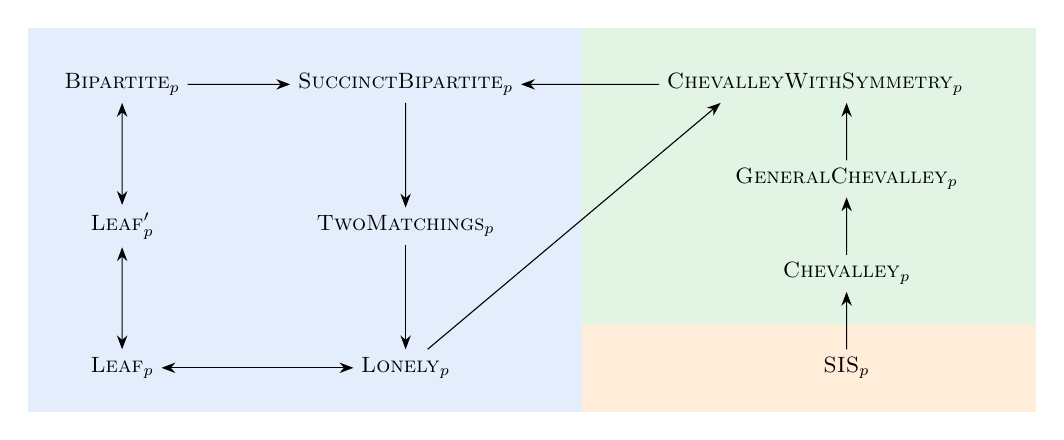
\begin{tikzpicture}[scale=0.8, transform shape]
	\def\hgap{2}
	\def\vgap{2.25}
	\draw[fill=Gblue!15, draw=none] (-7,2.4*\vgap) rectangle (1.8,-0.7);
	\draw[fill=Ggreen!15, draw=none] (9,2.4*\vgap) rectangle (1.8,-0.7);
	\draw[fill=orange!15, draw=none] (9,0.3*\vgap) rectangle (1.8,-0.7);
	\node (bip) at (-5.5,2*\vgap) {$\bipartite_p$};
	\node (leaf) at (-5.5,0) {$\leaf_p$};
	\node (leaf-p) at (-5.5,\vgap) {$\leaf'_p$};
	\node (lone) at (-1,0) {$\lonely_p$};
		\node (sbip) at (-1,2*\vgap) {$\sucBipartite_p$};
	\node (twomat) at (-1,\vgap) {$\twoMatchings_p$};

	\def\vgap{1.5}
	\node (combCh) at (5.5,4.5) {$\cChevalley_p$};
	\node (labelCh) at (6,4.5-\vgap) {$\lChevalley_p$};
	\node (Ch) at (6, 4.5-2*\vgap) {$\Chevalley_p$};
	\node (SIS) at (6, 4.5-3*\vgap) {$\sis_p$};

	\path[{Stealth[length=5pt]}-{Stealth[length=5pt]},line width=.4pt,black]
	(bip) edge (leaf-p)
	(leaf-p) edge (leaf)
	(leaf) edge (lone);

	\path[-{Stealth[length=5pt]},line width=.4pt,black]
	(bip) edge (sbip)
	(sbip) edge (twomat)
	(twomat) edge (lone)
	(lone) edge[bend right=0] ([shift={(-1.5,0)}]combCh.south)
	(combCh) edge (sbip)
	(labelCh) edge ([shift={(0.5,0)}]combCh.south)
	(Ch) edge (labelCh)
	(SIS) edge (Ch);
	\end{tikzpicture}
	\caption{Total search problems studied in this work. An arrow
	$A \rightarrow B$ denotes a reduction $A \reducible B$ that we establish.
	Problems in the \textcolor{Gblue}{blue} region are non-natural problems,
	which are all complete for $\PPA_p$. Problems in the
	\textcolor{Ggreen}{green} region are natural problems of which
	$\cChevalley_p$ is the one we show to be $\PPA_p$--complete. The problem
	in the \textcolor{orange}{orange} region is a cryptographically relevant problem.
				}
	\label{fig:ppa-landscape}
\end{figure}
 

\setcounter{section}{2}
\setcounter{theorem}{10}
\section{Characterization via Primes} \label{sec:characterization}

In this section we prove \autoref{thm:prime-characterization}, namely $\PPA_q = \amp_{p|q}\, \PPA_p$. The theorem follows by combining the following two ingredients.
\begin{itemize}[leftmargin=1.5cm,itemsep=3pt]
\item[\secref{sec:coprime}:]
$\PPA_{q r} = \PPA_q\bamp\PPA_r$ for any coprime $q$ and $r$.
\item[\secref{sec:prime-power}:]
$\PPA_{p^k} = \PPA_p$ for any prime power $p^k$.
\end{itemize}

\subsection{Coprime case} \label{sec:coprime}
\paragraph{\boldmath$\PPA_{qr} \supseteq \PPA_q \bamp\PPA_r$.}
We show that $\lonely_q \bamp\lonely_r$ reduces to $\lonely_{qr}$. Recall that an instance of $\lonely_q \bamp\lonely_r$ is a tuple $(C,V^*, b)$ where $(C,V^*)$ describes an instance of either $\lonely_q$ or $\lonely_r$ as chosen by $b\in\{0,1\}$. Suppose wlog that $b=0$, so the input encodes a $q$-dimensional matching $G = (V,E)$ over $V = [q]^n$ with designated vertices $V^*\subseteq V$, $|V^*| \not\equiv 0 \mod{q}$. We can construct a $qr$-dimensional matching $\overline{G} = (\overline{V},\overline{E})$ on vertices $\overline{V}\coloneqq V \times [r]$ as follows: For every hyperedge $e \coloneqq \set{v_1, \ldots, v_q} \in E$, we include the hyperedge $e \times [r]$ in $\overline{E}$. We let the designated vertices of $\overline{G}$ be $\overline{V}^* \coloneqq V^* \times [r]$. Note that $|\overline{V}^*| \not\equiv 0 \mod{qr}$. It is easy to see that a vertex $(v,i)$ is isolated in $G'$ iff $v$ is isolated in $G$. This completes the reduction since $\overline{V}$ is efficiently indexable, and the neighbors of any vertex in $\overline{V}$ are locally computable using black-box access to $C$. 

\paragraph{\boldmath $\PPA_{qr} \subseteq \PPA_q \bamp\PPA_r$.}
We show that $\bipartite_{qr}$ reduces to $\bipartite_q \bamp\bipartite_r$. Our input instance of $\bipartite_{qr}$ is a circuit $C : \bit^n \to (\bit^n)^k$ that encodes a bipartite graph $G = (V\cup U, E)$ with a designated node $v^* \in V$. If $\deg(v^*) \equiv 0 \mod{qr}$, then we already have solved the problem and no further reduction is necessary. Otherwise, if $\deg(v^*) \not\equiv 0 \mod{qr}$, we have, by the coprime-ness of $q$ and $r$, that either $\deg(v^*) \not\equiv 0 \mod{q}$ or $\deg(v^*) \not\equiv 0 \mod{r}$. In the first case (the second case is analogous), we can simply view $(G,v^*)$ as an instance of $\bipartite_q$, since vertices with degree $\not\equiv 0 \mod{q}$ in $G$ are also solutions to $\bipartite_{qr}$.

\subsection{Prime power case} \label{sec:prime-power}

$\PPA_{p^k} \supseteq \PPA_{p}$ follows immediately from our proof of $\PPA_{qr} \supseteq \PPA_q \bamp\PPA_r$, which didn't require that $q$ and $r$ be coprime. It remains to show $\PPA_{p^k} \subseteq \PPA_{p}$. We exploit the following easy fact.

\begin{fact}\label{fact:primes}
For all primes $p$, it holds that,\vspace*{-1mm}
\begin{align}
\text{for integers } t, c > 0: && \binom{c \cdot p^{t}}{p^t} \equiv 0 \mod{p} &\quad \text{if and only if }\ c \equiv 0 \mod{p}\label{eq:lucas-1}\\
\text{for integer } k > 0: && \binom{p^k}{i} \equiv 0 \mod{p} &\quad \text{for all }\ 0 < i < p^k\label{eq:lucas-2}
\end{align}

\end{fact}

\begin{figure}[t]
\centering
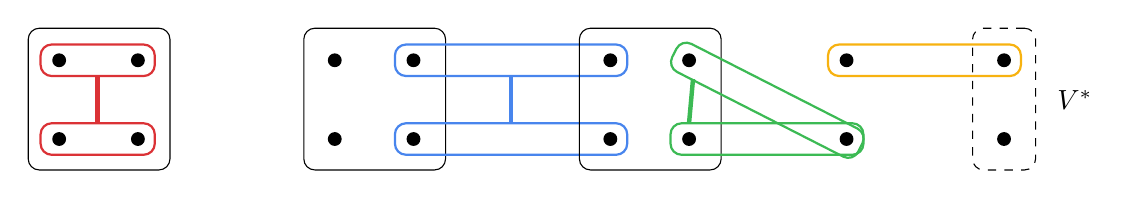
\begin{tikzpicture}
\tikzset{
	vert/.style = {circle, fill=black, minimum size=5pt, inner sep=0pt, outer sep=0pt},
	hedge/.style = {rectangle, rounded corners=4pt, above right, draw, minimum height=1.8cm, minimum width=1.8cm},
	medge/.style = {rectangle, rounded corners=4pt, draw, minimum height=0.4cm, minimum width=1.45cm, thick, right}
}
\node[vert] (A0) at (0,0) {};
\node[vert] (A1) at ([shift={(1,0)}]A0) {};
\node[vert] (A2) at ([shift={(1,1)}]A0) {};
\node[vert] (A3) at ([shift={(0,1)}]A0) {};
\node[hedge] at ([shift={(-0.4,-0.4)}]A0) {};
\node[medge, minimum width=1.45cm, draw=Gred] (A01) at ([shift={(-0.25,0)}]A0) {};
\node[medge, minimum width=1.45cm, draw=Gred] (A23)at ([shift={(-0.25,0)}]A3) {};
\draw[ultra thick, Gred] (A01) -- (A23);

\node[vert] (B0) at ([shift={(3.5,0)}]A0) {};
\node[vert] (B1) at ([shift={(1,0)}]B0) {};
\node[vert] (B2) at ([shift={(1,1)}]B0) {};
\node[vert] (B3) at ([shift={(0,1)}]B0) {};
\node[hedge] at ([shift={(-0.4,-0.4)}]B0) {};
\node[medge, minimum width=2.95cm, draw=Gblue] (B1C0) at ([shift={(-0.25,0)}]B1) {};
\node[medge, minimum width=2.95cm, draw=Gblue] (B2C3)at ([shift={(-0.25,0)}]B2) {};
\draw[ultra thick, Gblue] (B1C0) -- (B2C3);

\node[vert] (C0) at ([shift={(3.5,0)}]B0) {};
\node[vert] (C1) at ([shift={(1,0)}]C0) {};
\node[vert] (C2) at ([shift={(1,1)}]C0) {};
\node[vert] (C3) at ([shift={(0,1)}]C0) {};
\node[hedge] at ([shift={(-0.4,-0.4)}]C0) {};
\node[medge, minimum width=2.45cm, draw=Ggreen] (C1D0)at ([shift={(-0.25,0)}]C1) {};
\node[medge, minimum width=2.65cm, draw=Ggreen, rotate=-27] (C2D0)at ([shift={(-0.2,0.1)}]C2) {};
\draw[ultra thick, Ggreen, out=130, in=-100] ([shift={(0,0.12)}]C1.north) -- ([shift={(0.05,-0.15)}]C2.south);

\node[vert] (D0) at ([shift={(2,0)}]C1) {};
\node[vert] (D1) at ([shift={(2,0)}]D0) {};
\node[vert] (D2) at ([shift={(2,1)}]D0) {};
\node[vert] (D3) at ([shift={(0,1)}]D0) {};
\node[medge, minimum width=2.45cm, draw=Gyellow] (D1D2)at ([shift={(-0.25,0)}]D3) {};

\node[rectangle, rounded corners=4pt, above, draw, minimum height=1.8cm, minimum width=0.8cm, dashed] at ([shift={(0,-0.4)}]D1) {};
\node at ([shift={(0.9,0.5)}]D1) {$V^*$};

\end{tikzpicture}
\caption{Illustration of the proof of $\PPA_{p^k} \subseteq \PPA_{p}$ for $p=2$, $k=2$, $n=2$, $t=1$. In black, we indicate the $4$-dimensional matching $G$. In color, we highlight some of the vertices of $\overline{G}$ and the edges between them. The vertices of $\overline{G}$ in \textcolor{Gred}{red}, \textcolor{Gblue}{blue} and \textcolor{Ggreen}{green} are paired up and hence are non-solutions; whereas the vertex in \textcolor{Gyellow}{yellow} is isolated and not in $\overline{V}^*$ and hence a solution.}
\label{fig:ppa-prime-pow}
\end{figure}

\noindent We reduce $\lonely_{p^k}$ to $\lonely_p$. Our instance of $\lonely_{p^k}$ is $(C,V^*)$ where $C$ implicitly encodes a ${p^k}$-dimensional matching $G = (V = [p^k]^n, E)$ and a designated vertex set $V^* \subseteq V$ such that $|V^*| \not\equiv 0 \mod{p^k}$.

Let $p^t$, $0 \le t < k$, be the largest power of $p$ that divides $|V^*|$. Through local operations we construct a $p$-dimensional matching hypergraph $\overline{G} = (\overline{V}, \overline{E})$ over vertices $\overline{V} \coloneqq \binom{V}{p^t}$ (set of all size-$p^t$ subsets of $V$) with designated vertices $\overline{V}^*\coloneqq\binom{V^*}{p^t}$. From \eqnref{eq:lucas-1}, we get that $|\overline{V}| \equiv 0 \mod{p}$ and $|\overline{V}^*| \not\equiv 0 \mod{p}$.

We will describe an algorithm that on vertex $\overline{v} \in \overline{V}$ outputs a hyperedge of $p$ vertices that contains $\overline{v}$ (if any). To this end, first fix an algorithm that for any set $e \coloneqq \set{u_1, \ldots, u_{p^k}} \subseteq V$ and for any $1 \le i \le p^t$, computes some ``canonical'' partition of the set $\binom{e}{i}$ into subsets of size $p$, and moreover assigns a canonical cyclic order within each such subset. This is indeed possible because of \eqnref{eq:lucas-2}, since $t < k$.\\[-0.2cm]

\noindent Given a vertex $\overline{v} \coloneqq \set{v_1, \ldots, v_{p^t}} \in \overline{V}$,\vspace{-0.2cm}
\begin{itemize}[label=$\triangleright$,leftmargin=0.6cm]
\item Compute all edges $e_1, \ldots, e_\ell \in E$ that include some $v \in \overline{v}$.
\item For edge $e_j$, define $S_j \coloneqq e_j \cap \overline{v}$ and let $S_j^1, \ldots, S_j^{p-1}$ be the remaining subsets in the same partition as $S_j$ in the canonical partition of $\binom{e_j}{|S_j|}$, listed in the canonical cyclic order starting at $S_j$. Also, let $S_0$ be the set of untouched vertices in $\overline{v}$. Observe that $\overline{v} = S_0 \cup S_1 \cup \ldots \cup S_\ell$.
\item Output neighbors of $\overline{v}$ as the vertices $\overline{v}_1, \ldots, \overline{v}_{p-1}$ where $\overline{v}_i \coloneqq S_0 \cup S_1^i \cup \ldots \cup S_{\ell}^i$.
\end{itemize}

\noindent It is easy to see that $\overline{v}$ is isolated in $\overline{G}$ iff all $v \in \overline{v}$ are isolated in $G$. Moreover, any isolated vertex in $\overline{V} \smallsetminus \overline{V}^*$ contains at least one isolated vertex in $V \smallsetminus V^*$; and a non-isolated vertex in $\overline{V}^*$ contains at least one non-isolated vertex in $V^*$ (in fact $p^t$ many).

The edges of $\overline{G}$ can indeed be computed efficiently with just black-box access to $C$. In order to complete the reduction, we only need that $\overline{V}$ is efficiently indexable. This is indeed standard; see \cite[\S2.3]{r31} for a reference. See \autoref{fig:ppa-prime-pow} for an illustration of the proof.

\begin{remark}
Note that the size of the underlying graph blows up polynomially in our reduction. We do not know whether a reduction exists that avoids such a blow-up, although we suspect that the techniques of \cite{r6} can be used to show that some blow-up is necessary for black-box reductions.
\end{remark}


 

\appendix
\setcounter{section}{0}
\setcounter{theorem}{46}
\section{Appendix: Reductions Between Complete Problems}
\label{sec:equivalences}

In order to prove \autoref{thm:PPAqEquivalentProblems}, we introduce an additional problem that will serve as intermediate problem in our reductions.\\[1mm]


\noindent
\begin{minipage}{\linewidth}
\begin{definition}
	\label{def:leaf-prime} \contour{black}{($\leaf'_q$)}\vspace{-5pt}
	\begin{itemize}[leftmargin=2.15cm,itemsep=4pt]
		\item[\slshape Principle:] Same as $\leaf_q$, but degrees are allowed to be larger (polynomially bounded).
		\item[\slshape Object:] $q$-uniform hypergraph $G = (V, E)$. Designated vertex $v^* \in V$.
		\item[\slshape Inputs:] $\triangleright$ $C:\bit^n \to (\bit^{nq})^k$, with $(\bit^{nq})^k$ interpreted as $k$ many $q$-subsets of $\bit^n$\\
	$\triangleright$ $v^* \in \bit^n$ (usually $0^n$)
		\item[\slshape Encoding:] $V\coloneqq\bit^n$.\\
	For distinct $v_1, \ldots, v_q$, edge $e\coloneqq\set{v_1, \ldots, v_q}\in E$ if $e \in C(v)$ for all $v \in e$
		\item[\slshape Solutions:] $v^*$ if $\deg(v) \equiv 0 \mod{q}$ and\\
	$v \ne v^*$ if $\deg(v) \not\equiv 0 \mod{q}$
	\end{itemize}
\end{definition}
\end{minipage}\vspace{5mm}


\begin{proof}[Proof of \autoref{thm:PPAqEquivalentProblems}]
We show the following inter-reducibilities: (1) $\leaf_q \asymp \leaf_q'$, (2) $\leaf_q' \asymp \bipartite_q$ and (3) $\leaf_q \asymp \lonely_q$.

\medskip

\parasc{(1a) $\boldsymbol{\leaf_q \reducible \leaf_q'}$} Each instance of $\leafq$ is trivially an instance of $\leaf'_q$.

\medskip

\parasc{(1b) $\boldsymbol{\leaf'_q \reducible \leafq}$.} We start with a $\leaf'_q$ instance $(C, v^*)$, where $C$ encode a $q$-uniform hypergraph $G = (V, E)$ with degree at most $k$. Let $t = \ceil{k/q}$. We construct a $\leaf_q$ instance encoding a hypergraph $\overline{G} = (\overline{V}, \overline{E})$ on vertex set $\overline{V}\coloneqq V \times [t]$, intuitively making $t$ copies of each vertex.

In order to locally compute hyperedges, we first fix a canonical algorithm that for any vertex $v$ and any edge $e \in E$ incident on $v$, assigns it a label $\ell_v(e) \in [t]$, with at most $q$ edges mapping to the same label --- e.g. sort all edges incident on $v$ in lexicographic order and bucket them sequentially in at most $t$ groups of at most $q$ each. Note that we can ensure that for any vertex $v$ at most one label gets mapped to by a non-zero, non-$q$ number of edges. Moreover, if $\deg(v) \equiv 0 \mod{q}$, then exactly $q$ or $0$ edges are assigned to any label.

We'll assume that $\deg(v^*) \not\equiv 0 \mod{q}$, as otherwise, a reduction wouldn't be necessary. We let $(v^*, \ell^*)$ be the designated vertex of the $\leaf_q$ instance, where $\ell^*$ is the unique label that gets mapped to by a non-zero, non-$q$ number of edges incident on $v^*$.

For any vertex $(v, i) \in \overline{V}$, we assign it at most $q$ edges as follows: For each edge $e = \set{v_1, \ldots, v_q}$ such that $\ell_v(e)=i$, the corresponding hyperedge of $(v,i)$ is ${(v_1, \ell_{v_1}(e)), \ldots, (v_q, \ell_{v_q}(e))}$. It is easy to see that the designated vertex $(v^*, \ell^*)$ indeed has non-zero, non-$q$ degree. Moreover, a vertex $\deg(v,i) \notin \set{0, q}$ in $\overline{G}$ only if $v$ has a non-multiple-of-$q$ degree in $G$. Thus, solutions to the $\leaf_q$ instance naturally maps to solutions to the original $\leaf_q'$ instance.

By \autoref{rem:simplifications}, this completes the reduction since the edges are locally computable with black-box access to $C$ and $\overline{V}$ is efficiently indexable.

\medskip

\parasc{(2a) $\boldsymbol{\leaf'_q \reducible \bipartiteq}$.}
We start with a $\leaf'_q$ instance $(C, v^*)$, where $C$ encode a $q$-uniform hypergraph $G = (V, E)$. We construct a $\bipartite_q$ instance encoding a graph $\overline{G} = (\overline{V} \cup \overline{U}, \overline{E})$ such that $\overline{V} = V$ and $\overline{U} = \binom{V}{q}$, i.e. all $q$-sized subsets of $V$. We include the edge $(v,e) \in \overline{E}$ if $e \in E$ is incident on $v$. The designated vertex for the $\bipartite_q$ instance is $v^*$ in $\overline{V}$.

Clearly, all vertices $e \in \overline{U}$ have degree either $q$ or $0$. For any $v \in \overline{V}$, the degree of $v$ in $\overline{G}$ is same as its degree in $G$. Thus, any solution to the $\bipartite_q$ instance immediately gives a solution to the original $\leaf'_q$ instance. By \autoref{rem:simplifications}, this completes the reduction since the edges are locally computable with black-box access to $C$ and $\overline{V}$ and $\overline{U}$ are efficiently indexable (cf. \cite[\S2.3]{r31} for efficiently indexing $\overline{U}$).

\medskip

\parasc{(2b) $\boldsymbol{\bipartiteq \reducible \leaf'_q}$.} We start with a $\bipartite_q$ instance $(C, v^*)$ encoding a bipartite graph $\calG = (V \cup U,E)$ with maximum degree of any vertex being at most $k$. We construct a $\leaf'_q$ instance encoding a hypergraph $\overline{G} = (\overline{V}, \overline{E})$ such that $\overline{V} = V$ with designated vertex $v^*$.

First, we fix a canonical algorithm that for any vertex $u \in U$ with $\deg_{G}(u) \equiv 0 \mod{q}$ produces a partition of it's neighbors with $q$ vertices of $V$ in each part. Now, the set of $q$-uniform hyperedges incident on any vertex $v \in \overline{V}$ in $\overline{E}$ can be obtained as: for all neighbors $u$ of $v$, with $\deg_G(u) \equiv 0 \mod{q}$, we include a hyperedge consisting of all vertices in the same partition as $v$ among the neighbors of $u$ (we ignore neighbors $u$ with $\deg(u) \not\equiv 0 \mod{q}$).

Observe that $\deg_{\overline{G}}(v) \le \deg_{G}(v)$ and equality holds if and only if all neighbors of $v$ in $G$ have degree $\equiv 0 \mod{q}$. Hence for any $v \in \overline{V}$, if $\deg_{\overline{G}}(v) \ne \deg_G(v) \mod{q}$, then there exists a neighbor $u \in U$ of $v$ in $G$ such that $\deg(u) \not\equiv 0 \mod{q}$. Thus, if $v = v^*$ and $\deg_{\overline{G}}(v^*) \equiv 0 \mod{q}$, then either $\deg_G(v) \equiv 0 \mod{q}$ or we can find a neighbor $u$ of $v$ in $G$ with $\deg(u) \not\equiv 0 \mod{q}$. Similarly if for some $v \ne v^*$, we have $\deg_{\overline{G}}(v^*) \not\equiv 0 \mod{q}$, then either $\deg_G(v) \not\equiv 0 \mod{q}$ or we can find a neighbor $u$ of $v$ in $G$ with $\deg(u) \not\equiv 0 \mod{q}$. Thus, any solution to the $\leaf'_q$ instance gives us a solution to the original $\bipartite_q$ instance. This completes the reduction since $\overline{V} = \bit^n$ and the edges are locally computable with black-box access to $C$.

\medskip

\parasc{(3a) $\boldsymbol{\leaf_q \reducible \lonely_q}$.} We start with a $\leaf_q$ instance $(C, v^*)$, where $C$ encode a $q$-uniform hypergraph $G = (V, E)$ with degree at most $q$. If $\deg_G(v^*) = q$ or $0$, then we don't need any further reduction. Else, we construct a $\lonely_q$ instance encoding a $q$-dimensional matching $\overline{G} = (\overline{V}, \overline{E})$ on vertex set $\overline{V} = V \times [q]$. The designated vertices will be $V^* = \set{(v,q-i) : 1 \le i \le q - \deg(v^*)}$. Note that, $|V^*| = q - \deg_G(v^*)$ and hence $1 \le |V^*| \le q-1$.

In order to locally compute hyperedges, we first fix a canonical algorithm that for any vertex $v$ and any edge $e \in E$ incident on $v$, assigns it a unique label $\ell_v(e) \in [q]$ --- e.g. sort all edges incident on $v$ in lexicographic order and label them sequentially in $[q]$. In fact, we can ensure that an edge incident on $v$ get labeled within $\set{1, \ldots, \deg_G(v)}$.

For any vertex $(v, i) \in \overline{V}$, we assign it at most one hyperedge as follows:
\begin{itemize}[label=$\triangleright$]
\item If $\deg_G(v) = 0$, we include the hyperedge $\set{(v,i) : i \in [q]}$.
\item Else if $\deg_G(v) \ge i$, then for edge $e = \set{v_1, \ldots, v_q}$ incident on $v$ such that $\ell_v(e)=i$, the corresponding hyperedge of $(v,i)$ is ${(v_1, \ell_{v_1}(e)), \ldots, (v_q, \ell_{v_q}(e))}$.
\item Else if $0 < \deg_G(v) < i$, we leave it isolated.
\end{itemize}

It is easy to see that our definition of hyperedges is consistent and that the designated vertices $V^*$ are indeed isolated. Moreover, a vertex $(v,i)$ is isolated in $\overline{G}$ only if $1 \le \deg_G(v)\le q-1$. Thus, solutions to the $\leaf_q$ instance naturally maps to solutions to the original $\leaf_q'$ instance.

By \autoref{rem:simplifications}, this completes the reduction since the edges are locally computable with black-box access to $C$ and $\overline{V}$ is efficiently indexable.

\medskip

\parasc{(3b) $\boldsymbol{\lonely_q \reducible \leaf_q}$.} We start with a $\lonely_q$ instance $(C, V^*)$, where $C$ encode a $q$-dimensional matching $G = (V, E)$. We construct a $\leaf_q$ instance encoding a $q$-uniform hypergraph $\overline{G} = (\overline{V}, \overline{E})$ on vertex set $\overline{V}$ that will be specified shortly. We describe the hyperedges in $\overline{G}$ and it'll be clear how to compute the hyperedges for any vertex locally with just black-box access to $C$.

We start with $\overline{V} = V$. Our goal is to transform all vertices of degree $1$ to degree $q$, while ensuring that vertices of degree $0$ are mapped to vertices of degree not a multiple of $q$. Towards this goal we let $\overline{E}$ to be set of edges in $E$ in addition to $q-1$ canonical $q$-dimensional matchings over $V$. For example, for a vertex $v \coloneqq (x_1, \ldots, x_n) \in V = [q]^n$, the corresponding edges in $\overline{E}$ include an edge in $E$ (if any) and edges of the type $e_i = \set{(x_1, \dots, x_{i-1}, j, x_{i+1}, \dots, x_n) : j \in [q]}$ for $i \in [q-1]$ (note, this requires us to assume $n \geq q-1$). Adding the $q-1$ matchings increases the degree of each vertex by $q-1$. Therefore, vertices with initial degree $1$ now have degree $q$ and vertices with initial degree $0$ now have degree $q-1$. However, a couple of issues remain in order to complete the reduction, which we handle next.

{\em Multiplicities.} An edge $e \in E$ might have gotten added twice, if it belonged to one of the canonical matchings. To avoid this issue altogether, instead of adding edges directly on $V$, we augment $\overline{V}$ to become $\overline{V} \coloneqq V \cup \inparen{\binom{V}{q} \times [q-1]}$, i.e. in addition to $V$, we have $q-1$ vertices for every potential hyperedge of $G$. For any edge $e\coloneqq\set{v_1, \ldots, v_q} \in E$, instead of adding it directly in $\overline{G}$, we add hyperedge $\set{v, (e,1), (e,2), \ldots, (e,q-1)}$ for each $v \in e$. Note that, all vertices $(e,i) \in \binom{V}{q} \times [q-1]$ have degree $q$ if $e \in E$ and degree $0$ if $e \notin E$, so they are non-solutions for the $\leaf_q$ instance. For vertices in $V$, we still have as before that vertices with initial degree $1$ now have degree $q$ and vertices with initial degree $0$ now have degree $q-1$.

{\em Designated vertex.} In a $\leaf_q$ instance, we need to specify a single designated vertex $v^* \in \overline{V}$. If the $\lonely_q$ instance had a single designated vertex then we would be done. However, in general it is not possible to assume this (for non-prime $q$). Nevertheless, we provide a way to get around this. We augment $\overline{V}$ with $t = (q-1)(q-k) + 1$ additional vertices to become $\overline{V} \coloneqq V \cup  \inparen{\binom{V}{q} \times [q-1]} \cup \set{w_{i,j} : i \in [q-k],\ j \in [q-1]} \cup \set{v^*}$, where $v^*$ will eventually be the single designated vertex for the $\leaf_q$ instance.

Let $V^* = \set{u_1, \ldots, u_k} \subseteq V$ be the set of designated vertices in the $\lonely_q$ instance (note $1 \le k < q$). So far, note that $\deg_{\overline{G}}(u_i) = q-1$. The only new hyperedges we add will be among $u_i$'s, $w_{i,j}$'s and $v^*$, in such a way that $\deg_{\overline{G}}(u_i)$ will become $q$, the degree of all $w_{i,j}$'s will also be $q$ and degree of $v^*$ will be $q-k$.
\begin{itemize}[label=$\triangleright$, itemsep=3pt]
\item For each $u \in V^*$, include $\set{u, w_{1,1}, \ldots, w_{1,q-1}}$. So far, $\deg_{\overline{G}}(u) = q$ and $\deg_{\overline{G}}(w_{1,j}) = k$.
\item For each $j \in [q-1]$ and each $i \in \set{2, \ldots, q-k}$, include $\set{w_{1,j}, w_{i,1}, \ldots, w_{i,q-1}}$.\\
So far, $\deg_{\overline{G}}(w_{i,j}) = q-1$ for all $(i,j) \in [q-k] \times [q-1]$.
\item Finally, for each $(i,j) \in [q-k] \times [q-1]$, include $\set{v^*, w_{i,1}, \ldots, w_{i,q-1}}$.\\
Now, $\deg_{\overline{G}}(w_{i,j}) = q$ for all $(i,j) \in [q-k] \times [q-1]$ and $\deg_{\overline{G}}(v^*) = q-k$.
\end{itemize}

Thus, we have finally reduced to a $\leaf_q$ instance encoding the graph $\overline{G} = (\overline{V}, \overline{E})$ with $\overline{V} \coloneqq V \cup  \inparen{\binom{V}{q} \times [q-1]} \cup \set{w_{i,j} : i \in [q-k],\ j \in [q-1]} \cup \set{v^*}$. By \autoref{rem:simplifications}, this completes the reduction, since $\overline{V}$ is efficiently indexable (again, see \cite{r31} for a reference on indexing $\binom{V}{q}$) and the edges are locally computable using black-box access to $C$.
\end{proof}


\begin{thebibliography}{37}
\bibitem{r1} James Aisenberg, Maria Luisa Bonet, and Sam Buss. 2-d tucker is PPA complete. Electronic Colloquium on Computational Complexity (ECCC), 22:163, 2015. URL: http://eccc.hpi-web. de/report/2015/163.
\bibitem{r2} Noga Alon. Splitting necklaces. Advances in Mathematics, 63(3):247–253, 1987. doi:10.1016/ 0001-8708(87)90055-7.
\bibitem{r3} Noga Alon, Shmuel Friedland, and Gil Kalai. Regular subgraphs of almost regular graphs. Journal of Combinatorial Theory, Series B, 37(1):79–91, 1984.
\bibitem{r4} Noga Alon and Douglas B. West. The Borsuk-Ulam theorem and bisection of necklaces. Proceedings of the American Mathematical Society, 98(4):623–628, 1986. doi: 10.1090/S0002-9939-1986-0861764-9.
\bibitem{r5} Paul Beame, Stephen A. Cook, Jeff Edmonds, Russell Impagliazzo, and Toniann Pitassi. The relative complexity of NP search problems. J. Comput. Syst. Sci., 57(1):3–19, 1998. doi:10.1006/jcss.1998.1575.
\bibitem{r6} Paul Beame and Søren Riis. More on the relative strength of counting principles. In Proceedings of the DIMACS Workshop on Proof Complexity and Feasible Arithmetics, volume 39, pages 13–35, 1998.
\bibitem{r7} Richard Beigel and John Gill. Counting classes: Thresholds, parity, mods, and fewness. Theor. Comput. Sci., 103(1):3–23, 1992. doi:10.1016/0304-3975(92)90084-S.
\bibitem{r8} Aleksandrs Belovs, Gábor Ivanyos, Youming Qiao, Miklos Santha, and Siyi Yang. On the polynomial parity argument complexity of the combinatorial nullstellensatz. In 32nd Computational Complexity Conference, CCC 2017, July 6-9, 2017, Riga, Latvia, pages 30:1– 30:24, 2017. doi:10.4230/LIPIcs.CCC.2017.30.
\bibitem{r9} Nir Bitansky, Omer Paneth, and Alon Rosen. On the cryptographic hardness of finding a nash equilibrium. In 2015 IEEE 56th Annual Symposium on Foundations of Computer Science, pages 1480–1498. IEEE, 2015.
\bibitem{r10} Josh Buresh-Oppenheim and Tsuyoshi Morioka. Relativized NP search problems and propositional proof systems. In 19th Annual IEEE Conference on Computational Complexity (CCC 2004), 21-24 June 2004, Amherst, MA, USA, pages 54–67, 2004. doi: 10.1109/CCC.2004.1313795.
\bibitem{r11} Joshua Buresh-Oppenheim. On the TFNP complexity of factoring. Manuscript, 2006. URL: http://www.cs.toronto.edu/~bureshop/factor.pdf.
\bibitem{r12} Samuel R. Buss, Dima Grigoriev, Russell Impagliazzo, and Toniann Pitassi. Linear gaps between degrees for the polynomial calculus modulo distinct primes. J. Comput. Syst. Sci., 62(2):267–289, 2001. doi:10.1006/jcss.2000.1726.
\bibitem{r13} Samuel R. Buss and Alan S. Johnson. Propositional proofs and reductions between NP search problems. Ann. Pure Appl. Logic, 163(9):1163–1182, 2012. doi:10.1016/j.apal.2012.01.015.
\bibitem{r14} I. Bárány, S. B. Shlosman, and A. Szücs. On a topological generalization of a theorem of tverberg. Journal of the London Mathematical Society, s2-23(1):158–164, 1981. doi: 10.1112/jlms/s2-23.1.158.
\bibitem{r15} Claude Chevalley. Démonstration d’une hypothèse de m. artin. Abhandlungen aus dem Mathematischen Seminar der Universität Hamburg, 11(1):73–75, December 1935. doi:10. 1007/BF02940714.
\bibitem{r16} Arka Rai Choudhuri, Pavel Hubácek, Chethan Kamath, Krzysztof Pietrzak, Alon Rosen, and Guy N Rothblum. Finding a nash equilibrium is no easier than breaking fiat-shamir. In Proceedings of the 51st Annual ACM SIGACT Symposium on Theory of Computing, pages 1103–1114. ACM, 2019.
\bibitem{r17} Constantinos Daskalakis, Paul W. Goldberg, and Christos H. Papadimitriou. The complexity of computing a nash equilibrium. SIAM J. Comput., 39(1):195–259, 2009. doi:10.1137/ 070699652.
\bibitem{r18} Constantinos Daskalakis and Christos H. Papadimitriou. Continuous local search. In Proceedings of the Twenty-Second Annual ACM-SIAM Symposium on Discrete Algorithms, SODA 2011, San Francisco, California, USA, January 23-25, 2011, pages 790–804, 2011. doi:10.1137/1.9781611973082.62.
\bibitem{r19} Xiaotie Deng, Jack R. Edmonds, Zhe Feng, Zhengyang Liu, Qi Qi, and Zeying Xu. Understanding PPA-Completeness. In Ran Raz, editor, 31st Conference on Computational Complexity (CCC 2016), volume 50 of Leibniz International Proceedings in Informatics (LIPIcs), pages 23:1–23:25, Dagstuhl, Germany, 2016. Schloss Dagstuhl–Leibniz-Zentrum fuer Informatik. doi:10.4230/LIPIcs.CCC.2016.23.
\bibitem{r20} Aris Filos-Ratsikas and Paul W. Goldberg. Consensus halving is ppa-complete. In Proceedings of the 50th Annual ACM SIGACT Symposium on Theory of Computing, STOC 2018, Los Angeles, CA, USA, June 25-29, 2018, pages 51–64, 2018. doi:10.1145/3188745.3188880.
\bibitem{r21} Aris Filos-Ratsikas and Paul W. Goldberg. The complexity of splitting necklaces and bisecting ham sandwiches. In STOC (to appear), 2019. arXiv:1805.12559.
\bibitem{r22} C. Goldberg and D. West. Bisection of circle colorings. SIAM Journal on Algebraic Discrete Methods, 6(1):93–106, 1985. doi:10.1137/0606010.
\bibitem{r23} Mika Göös, Pritish Kamath, Robert Robere, and Dmitry Sokolov. Adventures in monotone complexity and TFNP. In 10th Innovations in Theoretical Computer Science Conference, ITCS 2019, January 10-12, 2019, San Diego, California, USA, pages 38:1–38:19, 2019. doi:10.4230/LIPIcs.ITCS.2019.38.
\bibitem{r24} Michelangelo Grigni. A sperner lemma complete for ppa. Information Processing Letters, 77(5-6):255–259, 2001.
\bibitem{r25} Alexandros Hollender. The classes PPA-k: Existence from arguments modulo k. In Ioannis Caragiannis, Vahab Mirrokni, and Evdokia Nikolova, editors, Web and Internet Economics, pages 214–227, Cham, 2019. Springer International Publishing.
\bibitem{r26} Emil Jerábek. Integer factoring and modular square roots. J. Comput. Syst. Sci., 82(2):380–394, 2016. doi:10.1016/j.jcss.2015.08.001.
\bibitem{r27} Alan S. Johnson. Reductions and propositional proofs for total NP search problems. UC San Diego Electronic Theses and Dissertations, 2011. URL: https://escholarship.org/uc/ item/89r774x7.
\bibitem{r28} David S. Johnson, Christos H. Papadimitriou, and Mihalis Yannakakis. How easy is local search? J. Comput. Syst. Sci., 37(1):79–100, 1988. doi:10.1016/0022-0000(88)90046-3.
\bibitem{r29} Ilan Komargodski, Moni Naor, and Eylon Yogev. White-box vs. black-box complexity of search problems: Ramsey and graph property testing. Journal of the ACM (JACM), 66(5):34, 2019.
\bibitem{r30} Pravesh K Kothari and Ruta Mehta. Sum-of-squares meets nash: lower bounds for finding any equilibrium. In Proceedings of the 50th Annual ACM SIGACT Symposium on Theory of Computing, pages 1241–1248. ACM, 2018.
\bibitem{r31} Donald L. Kreher and Douglas R. Stinson. Combinatorial Algorithms: Generation, Enumeration, and Search, volume 7 of Discrete Mathematics and Its Applications. CRC Press, 1998.
\bibitem{r32} Nimrod Megiddo and Christos H. Papadimitriou. On total functions, existence theorems and computational complexity. Theor. Comput. Sci., 81(2):317–324, 1991. doi:10.1016/ 0304-3975(91)90200-L.
\bibitem{r33} Christos H. Papadimitriou. On the complexity of the parity argument and other inefficient proofs of existence. J. Comput. Syst. Sci., 48(3):498–532, 1994. doi:10.1016/S0022-0000(05) 80063-7.
\bibitem{r34} Christian Reiher. On kemnitz’conjecture concerning lattice-points in the plane. The Ramanujan Journal, 13(1-3):333–337, 2007.
\bibitem{r35} Aviad Rubinstein. Settling the complexity of computing approximate two-player nash equilibria. In IEEE 57th Annual Symposium on Foundations of Computer Science, FOCS 2016, 9-11 October 2016, Hyatt Regency, New Brunswick, New Jersey, USA, pages 258–265, 2016.
\bibitem{r36} Katerina Sotiraki, Manolis Zampetakis, and Giorgos Zirdelis. Ppp-completeness with connections to cryptography. In 59th IEEE Annual Symposium on Foundations of Computer Science, FOCS 2018, Paris, France, October 7-9, 2018, pages 148–158, 2018. doi: 10.1109/FOCS.2018.00023.
\bibitem{r37} Ewald Warning. Bemerkung zur vorstehenden arbeit von herrn chevalley. Abh. Math. Sem. Univ. Hamburg, 11:76–83, 1936.
\end{thebibliography}
\end{document}
